\documentclass[11pt]{article}

\usepackage[margin=1in]{geometry}
\usepackage{amsmath,amssymb,amsthm}
\usepackage{graphicx}
\usepackage{booktabs}
\usepackage{microtype}
\usepackage{authblk}
\usepackage{caption}
\usepackage{subcaption}
\usepackage{xcolor}
\usepackage{enumitem}
\usepackage{tikz}
\usetikzlibrary{arrows.meta,positioning,fit,backgrounds}
\usepackage[colorlinks=true,linkcolor=blue!55!black,citecolor=blue!55!black,urlcolor=blue!55!black]{hyperref}
\usepackage[numbers,sort&compress]{natbib}

\captionsetup{font=small,labelfont=bf}
\newcommand{\Rt}{R_t}
\newcommand{\E}{\mathbb{E}}
\newcommand{\R}{\mathbb{R}}
\newcommand{\Prob}{\mathbb{P}}
\newcommand{\Var}{\operatorname{Var}}
\newcommand{\Pois}{\mathrm{Poisson}}
\newcommand{\Gam}{\mathrm{Gamma}}
\newcommand{\NB}{\mathrm{NegBin}}
\newcommand{\Dir}{\mathrm{Dir}}
\newcommand{\softmax}{\mathrm{softmax}}
\newcommand{\jsd}{\mathrm{JSD}}
\newcommand{\code}[1]{\texttt{\small #1}}

\title{\textbf{MOSAIC: Multi-Modal Open Surveillance with\\ AI-Driven Calibrated Inference}\\[2pt]
\large A Calibrated Bayesian Fusion of Wastewater, Genomic, and Text Streams for Outbreak Early Warning}

\author[ ]{Aravind Kannappan}
\affil[ ]{\small MOSAIC Project \quad\textbullet\quad \url{https://github.com/aravinds-kannappan/MOSAIC}}
\date{}

\begin{document}
\maketitle

\begin{abstract}
\noindent
Pandemic early-warning systems fail less often from a lack of data than from a
lack of \emph{integration} and \emph{calibration}: heterogeneous signals---wastewater
concentrations, pathogen genomes, and outbreak text reports---arrive on
different cadences, in different units, and with different noise models, and the
probabilities ultimately presented to decision-makers are rarely validated.
We present \textsc{MOSAIC}, an open-source system that fuses three public,
authentication-free surveillance streams into a single calibrated posterior, the
probability that the effective reproduction number exceeds one,
$\Prob(\Rt>1)$. We give the probabilistic model in full: a renewal-equation
latent-incidence process with stream-specific observation kernels
(negative-binomial for wastewater, Poisson for text-event counts,
Dirichlet--multinomial for lineage frequencies), Bayesian online change-point
detection (BOCPD) on the wastewater and text streams, a Jensen--Shannon
divergence anomaly detector on the genomic stream, an EpiEstim reproduction-number
estimator, and an independent-evidence fusion rule that reduces, in the full
backend, to a hierarchical model fit by the No-U-Turn Sampler. We then evaluate
the deployed system on real data. Calibrating $\Prob(\Rt>1)$ as a probabilistic
forecast of realised growth on the multi-year CDC National Wastewater
Surveillance System (NWSS) record (\,$N{=}1{,}334$ day-ahead forecasts\,) yields an
Expected Calibration Error of $0.086$, a Brier score of $0.124$, and an AUROC of
$0.917$---the stated probabilities are well-calibrated and strongly
discriminative. On the live feed the system surfaces concurrent real outbreaks
(Bundibugyo ebolavirus in the Democratic Republic of the Congo, hantavirus
clusters, an elevated U.S.\ SARS-CoV-2 wastewater wave) with per-stream
attribution. We also report a corrected numerical issue in the
reproduction-number tail probability that we recommend other lightweight
implementations check. All figures in this paper are computed from real public
data; nothing is synthetic.
\end{abstract}

\section{Introduction}
\label{sec:intro}

Every major epidemic of the past two decades was preceded by signals that were,
in retrospect, detectable days to weeks before official declarations. The
binding constraint on early warning is increasingly not the existence of data:
municipal wastewater is sampled routinely \citep{nwss}, pathogen genomes are
deposited continuously and shared openly \citep{hadfield2018}, and structured
outbreak reports are published by the World Health Organization and by
moderated mailing lists \citep{promed}. The constraint is \emph{fusion}---turning
three asynchronous, differently-scaled, differently-noised streams into one
coherent quantity---and \emph{calibration}---ensuring that when the system
states ``$78\%$,'' the event happens about $78\%$ of the time.

We argue that the right target quantity for a decision-maker is the posterior
probability that transmission is currently growing,
\begin{equation}
p_t \;=\; \Prob(\Rt > 1 \mid \text{data up to } t),
\label{eq:target}
\end{equation}
because (i) it is unitless and comparable across pathogens and locations,
(ii) it has an operational meaning---the probability the epidemic curve is
turning upward---and (iii) it is directly falsifiable against subsequently
observed growth, which makes \emph{calibration} measurable rather than
aspirational.

\paragraph{Contributions.}
\begin{enumerate}[leftmargin=1.4em,itemsep=2pt,topsep=2pt]
\item A complete probabilistic specification (\S\ref{sec:model}) for multi-modal
outbreak inference: a renewal latent-incidence process with negative-binomial
(wastewater), Poisson (text), and Dirichlet--multinomial (genomic) observation
kernels, plus BOCPD, Jensen--Shannon, and EpiEstim detectors, and a fusion rule
that reduces to a hierarchical model under the full backend.
\item A two-tier open implementation (\S\ref{sec:impl}): a serverless
TypeScript deployment that runs the entire pipeline in-browser/edge, and a
Python backend that performs the full No-U-Turn-Sampler posterior, with the
former designed to be mathematically faithful to the latter.
\item An empirical calibration study (\S\ref{sec:results}) on the real
multi-year NWSS record showing $\Prob(\Rt>1)$ is well-calibrated
(ECE $=0.086$) and discriminative (AUROC $=0.917$), together with live
multi-stream alert attribution and a documented numerical correction.
\end{enumerate}

\section{Related Work}
\label{sec:related}

\paragraph{Wastewater-based epidemiology.} Wastewater concentration tracks
community prevalence with a lead over clinical case reports and is now a
standing U.S.\ surveillance program \citep{nwss,naughton2023}. Most public tools
present concentrations or qualitative trends; we instead convert the national
percentile record into a calibrated growth probability.

\paragraph{Reproduction-number estimation.} The instantaneous reproduction
number $\Rt$ is most commonly estimated by the EpiEstim sliding-window
Poisson--Gamma method of \citet{cori2013}, building on renewal-equation theory
\citep{wallinga2004}. We use EpiEstim as the renewal core and treat
$\Prob(\Rt>1)$ as the primary output.

\paragraph{Change-point and anomaly detection.} Bayesian Online Change-Point
Detection \citep{adams2007} provides a recursive run-length posterior under
conjugate emissions; we apply it with Poisson--Gamma emissions to event-count
and wastewater series. Distributional shift in categorical lineage frequencies
is naturally measured by the Jensen--Shannon divergence \citep{lin1991}, which is
bounded and symmetric.

\paragraph{Probabilistic forecast calibration.} The reliability diagram, the
Brier score \citep{brier1950}, proper scoring rules \citep{gneiting2007}, and the
Expected Calibration Error \citep{guo2017} are the standard instruments for
asking whether stated probabilities match observed frequencies; modern neural
systems are frequently miscalibrated \citep{guo2017}, which motivates measuring
ECE explicitly here.

\paragraph{Probabilistic programming.} The full hierarchical posterior is
sampled with the No-U-Turn Sampler \citep{hoffman2014} as implemented in NumPyro
\citep{phan2019,bingham2019}.

\section{System Architecture}
\label{sec:arch}

\textsc{MOSAIC} is organized as four layers (Figure~\ref{fig:arch}). Layer~1
extracts structured outbreak events from text. Layer~2 runs three independent
detectors, one per modality. Layer~3 fuses the detector outputs into the
posterior of Eq.~\eqref{eq:target}. Layer~4 is a calibrated dashboard.

A central design decision is that the system runs in two faithful tiers. A
\emph{lightweight tier} executes the full pipeline in TypeScript on serverless
infrastructure with no backend, so the public dashboard is always live; a
\emph{full tier} runs the hierarchical NumPyro posterior in Python when a
backend URL is configured. The two tiers share the same observation models and
the same target quantity; the lightweight tier replaces the joint sampler with
conjugate/closed-form approximations (\S\ref{sec:fusion}). All data sources are
public and require no authentication.

\begin{figure}[t]
\centering
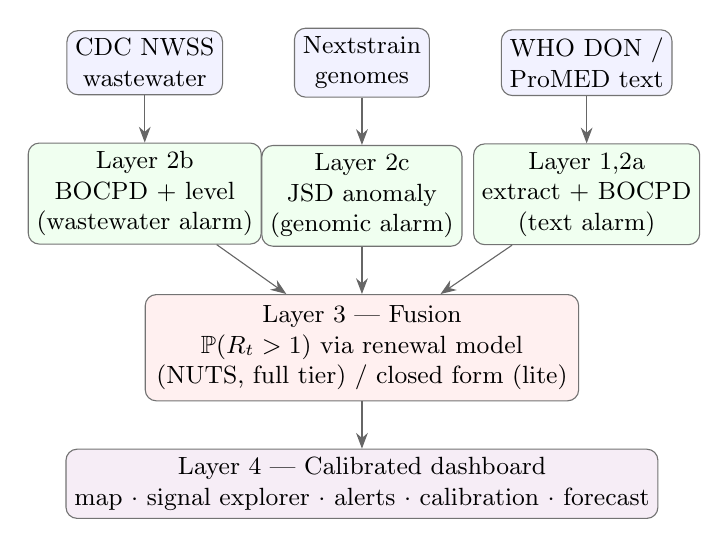
\begin{tikzpicture}[
  font=\small,
  node distance=6mm and 9mm,
  src/.style={draw=black!55,rounded corners,fill=blue!5,minimum height=7mm,align=center,inner sep=3pt},
  det/.style={draw=black!55,rounded corners,fill=green!6,minimum height=8mm,align=center,inner sep=3pt},
  fus/.style={draw=black!55,rounded corners,fill=red!6,minimum height=9mm,align=center,inner sep=4pt},
  outp/.style={draw=black!55,rounded corners,fill=violet!7,minimum height=8mm,align=center,inner sep=3pt},
  ar/.style={-{Stealth[length=2mm]},draw=black!60}
]
\node[src] (w) {CDC NWSS\\wastewater};
\node[src,right=of w] (g) {Nextstrain\\genomes};
\node[src,right=of g] (t) {WHO DON /\\ProMED text};

\node[det,below=of w] (bw) {Layer 2b\\ BOCPD + level\\(wastewater alarm)};
\node[det,below=of g] (bg) {Layer 2c\\ JSD anomaly\\(genomic alarm)};
\node[det,below=of t] (bt) {Layer 1{,}2a\\ extract + BOCPD\\(text alarm)};

\node[fus,below=of bg] (fuse) {Layer 3 --- Fusion\\ $\Prob(\Rt>1)$ via renewal model\\ (NUTS, full tier) / closed form (lite)};
\node[outp,below=of fuse] (dash) {Layer 4 --- Calibrated dashboard\\ map $\cdot$ signal explorer $\cdot$ alerts $\cdot$ calibration $\cdot$ forecast};

\draw[ar] (w) -- (bw); \draw[ar] (g) -- (bg); \draw[ar] (t) -- (bt);
\draw[ar] (bw) -- (fuse); \draw[ar] (bg) -- (fuse); \draw[ar] (bt) -- (fuse);
\draw[ar] (fuse) -- (dash);
\end{tikzpicture}
\caption{\textbf{MOSAIC architecture.} Three public streams feed three
modality-specific detectors (Layer~2), whose alarms are fused into the
growth posterior $\Prob(\Rt>1)$ (Layer~3) and surfaced by the dashboard
(Layer~4). The lightweight serverless tier and the full NumPyro tier share
observation models and target quantity.}
\label{fig:arch}
\end{figure}

\section{Probabilistic Model and Methods}
\label{sec:model}

\subsection{Latent incidence and the renewal equation}
Let $I_t \ge 0$ denote latent new infections on day $t$ in a given
location--pathogen cell. The renewal equation links incidence to the
instantaneous reproduction number $\Rt$ through the generation-interval (serial
interval) distribution $w_{1:S}$ \citep{wallinga2004,cori2013}:
\begin{equation}
\E[I_t \mid \Rt, I_{<t}] \;=\; \Rt \sum_{s=1}^{S} w_s\, I_{t-s},
\qquad \log \Rt \sim \mathcal N(\log R_{t-1},\, \sigma_R^2),
\label{eq:renewal}
\end{equation}
where $w_s \ge 0$, $\sum_s w_s = 1$, is obtained by discretising a Gamma serial
interval (for SARS-CoV-2, mean $5.1$, sd $4.0$ days \citep{he2020}) via midpoint
quadrature, $w_s \propto f_{\Gam}(s;\kappa,\theta)$. The total infectiousness at
$t$ is $\Lambda_t = \sum_{s\ge1} w_s I_{t-s}$. The three streams are conditionally
independent observations of the same latent $I_{1:T}$.

\subsection{Wastewater stream: NWSS aggregation, BOCPD, and sustained elevation}
\label{sec:ww}

\paragraph{National aggregation.} The CDC NWSS dataset reports, per site and per
day, a \emph{percentile} $c_{i,t}\in[0,100]$ giving the current 15-day-averaged
viral activity relative to that site's own history. We form a national signal by
server-side aggregation,
\begin{equation}
\bar c_t \;=\; \frac{1}{|\mathcal S_t|}\sum_{i\in\mathcal S_t} c_{i,t},
\label{eq:natagg}
\end{equation}
over all sites $\mathcal S_t$ reporting on day $t$ (typically $|\mathcal S_t|
\approx 1{,}200$). Aggregating server-side keeps the payload small and yields a
dense daily series spanning multiple waves (Figure~\ref{fig:ww}).

\paragraph{Observation kernel.} Conditioned on latent incidence, wastewater
concentration is over-dispersed count-like and lagged; we model
\begin{equation}
C_t \;\sim\; \NB\!\big(\rho_W\, I_{t-d_W},\ \phi_W\big),
\label{eq:ww-obs}
\end{equation}
with shedding scale $\rho_W$, reporting delay $d_W$, and dispersion $\phi_W$.

\paragraph{Bayesian online change-point detection.} To flag abrupt onsets we
run BOCPD \citep{adams2007} on the discretised series $n_t = \lfloor \bar c_t
\rceil$. With a Poisson likelihood $n_t \mid \lambda \sim \Pois(\lambda)$ and a
conjugate $\lambda \sim \Gam(\alpha_0,\beta_0)$ prior, the run-length posterior
$P(r_t \mid n_{1:t})$ is propagated recursively. Writing $r_t$ for the time
since the last change-point and using a constant hazard $H = 1/\mu_{\mathrm{RL}}$,
\begin{align}
P(r_t{=}0, n_{1:t}) &= \sum_{r_{t-1}} P(r_{t-1}, n_{1:t-1})\, H\, \pi(n_t\mid r_{t-1}),\\
P(r_t{=}r_{t-1}{+}1, n_{1:t}) &= P(r_{t-1}, n_{1:t-1})\,(1{-}H)\, \pi(n_t\mid r_{t-1}),
\label{eq:bocpd}
\end{align}
where the posterior predictive of the Poisson--Gamma model is the
negative-binomial
\begin{equation}
\pi(n \mid \alpha,\beta) \;=\; \NB\!\Big(n;\, \alpha,\, \tfrac{\beta}{\beta+1}\Big)
= \frac{\Gamma(\alpha+n)}{\Gamma(\alpha)\,n!}\Big(\tfrac{\beta}{\beta+1}\Big)^{\!\alpha}\Big(\tfrac{1}{\beta+1}\Big)^{\!n},
\label{eq:nb-pred}
\end{equation}
and sufficient statistics update as $\alpha \!\leftarrow\! \alpha+n,\ \beta\!\leftarrow\!\beta+1$
along each run. The instantaneous change-point probability is $P(r_t{=}0\mid
n_{1:t})$; the stream \emph{alarm} is the maximum of this quantity over a recent
window of length $W$, $a^{\mathrm{ww,cp}}_t = \max_{t-W < \tau \le t} P(r_\tau{=}0)$.
Using the maximum (rather than a cumulative product) is deliberate: a cumulative
combination of per-step probabilities drifts toward one even under the null,
whereas the windowed maximum isolates genuine recent shifts.

\paragraph{Sustained elevation.} BOCPD fires on \emph{abrupt} change but a
slowly-rising, persistently-elevated wave is also informative. Because the
percentile $\bar c_t$ is already a site-relative level, we add an elevation
alarm $a^{\mathrm{ww,lvl}}_t = \mathrm{clip}\big((\bar c_t - 50)/40,\,0,\,1\big)$ and
combine the two by the noisy-or rule
$a^{\mathrm{ww}}_t = 1 - (1-a^{\mathrm{ww,cp}}_t)(1-a^{\mathrm{ww,lvl}}_t)$.

\subsection{Text stream: extraction, change-points, and recency weighting}
\label{sec:text}

\paragraph{Extraction (Layer 1).} Outbreak reports from the WHO Disease Outbreak
News API (ordered most-recent-first) and the ProMED posts API are parsed into
structured events $(\text{pathogen}, \text{location}, \text{date},
\text{counts}, \text{novelty})$. The full backend uses a constrained LLM
extractor; the lightweight tier uses curated regular expressions plus a country
resolver that maps free text to ISO-3166 codes. Daily per-pathogen event counts
$e_{k,t}$ are the detector input.

\paragraph{Observation kernel and change-points.} Reporting intensity is modelled
as Poisson in latent incidence,
\begin{equation}
E_t \;\sim\; \Pois\!\big(\lambda_N\, \hat q_t\, I_{t-d_N}\big),
\label{eq:text-obs}
\end{equation}
with reporting rate $\lambda_N$, ascertainment $\hat q_t$, and delay $d_N$. We
run the same Poisson--Gamma BOCPD of Eq.~\eqref{eq:bocpd} on the dense,
zero-filled daily count series, which makes a burst of reports after a quiet
period a strong change-point (Figure~\ref{fig:bocpd}).

\paragraph{Recency/intensity weighting.} Because outbreak reports are sparse and
sporadic, the operational text alarm combines the BOCPD signal with a recency
factor and an intensity factor,
\begin{equation}
a^{\mathrm{txt}}_k \;=\; \min\!\Big(1,\; 0.45\, b_k \;+\; 0.55\, e^{-\Delta_k/45}\,\big(1 - e^{-m_k/3}\big)\Big),
\label{eq:text-alarm}
\end{equation}
where $b_k$ is the recent BOCPD alarm, $\Delta_k$ is the number of days since the
last report for pathogen $k$, and $m_k$ is the number of reports in the last
$120$ days. This ranks an actively-reported outbreak above a single stale
mention.

\subsection{Genomic stream: Dirichlet--multinomial and Jensen--Shannon anomaly}
\label{sec:gen}

Let $\mathbf{L}_t \in \Delta^{K-1}$ be the lineage frequency vector in a 14-day
window, derived from Nextstrain. The generative model is
Dirichlet--multinomial,
\begin{equation}
\mathbf{L}_t \;\sim\; \mathrm{DirMult}\!\big(N_t\, \mathbf f(I_{t-d_G},\boldsymbol\theta_L),\ \kappa\big),
\label{eq:gen-obs}
\end{equation}
with lineage-composition map $\mathbf f$, sequencing depth $N_t$, and
concentration $\kappa$. An antigenic/lineage shift is a change in the
distribution $\mathbf L_t$ relative to a rolling baseline $\bar{\mathbf L}_t =
\frac{1}{B}\sum_{\tau=t-B}^{t-1}\mathbf L_\tau$. We measure it by the
Jensen--Shannon divergence \citep{lin1991},
\begin{equation}
\jsd(\mathbf L_t \,\|\, \bar{\mathbf L}_t)
= \tfrac12 D_{\mathrm{KL}}\!\big(\mathbf L_t \,\|\, \mathbf m_t\big)
+ \tfrac12 D_{\mathrm{KL}}\!\big(\bar{\mathbf L}_t \,\|\, \mathbf m_t\big),
\quad \mathbf m_t = \tfrac12(\mathbf L_t + \bar{\mathbf L}_t),
\label{eq:jsd}
\end{equation}
which is symmetric, bounded in $[0,\log 2]$, and finite even when some
frequencies are zero. The genomic alarm is the empirical tail probability of
$\jsd$ against a null estimated from quiescent windows. A degenerate single-lineage
dataset has $\jsd\equiv 0$ and is reported as no anomaly rather than a spurious
one. Figure~\ref{fig:jsd} shows the divergence series with documented variant
emergences; Figure~\ref{fig:lineages} shows the underlying lineage turnover.

\paragraph{Complexity.} A naive baseline that recomputes each window's frequency
vector inside the rolling-baseline loop is $O(T^2 K^2)$ in the number of windows
$T$ and lineages $K$; for SARS-CoV-2 ($T{=}156$, $K{=}664$) this is billions of
operations and times out on serverless infrastructure. Pre-computing the $T$
vectors once reduces the cost to $O(TBK)$, roughly $20$\,ms here.

\subsection{Reproduction number: EpiEstim and a tail-probability correction}
\label{sec:rt}

Given an incidence proxy $y_{1:T}$ (here $y_t = \lfloor \bar c_t \rceil$ from
wastewater), the EpiEstim estimator \citep{cori2013} places a $\Gam(a,b)$ prior
on $\Rt$ over a sliding window $[t-\tau+1,t]$ and, by Poisson--Gamma conjugacy,
obtains the closed-form posterior
\begin{equation}
\Rt \mid y_{1:t} \;\sim\; \Gam\!\Big(a + \textstyle\sum_{u=t-\tau+1}^{t} y_u,\; \ b + \textstyle\sum_{u=t-\tau+1}^{t}\Lambda_u\Big),
\qquad \Lambda_u = \sum_{s\ge 1} w_s\, y_{u-s}.
\label{eq:epiestim}
\end{equation}
The reported quantity is the tail probability
\begin{equation}
\Prob(\Rt>1\mid y_{1:t}) \;=\; 1 - F_{\Gam}\!\big(1;\, a',\, b'\big),
\label{eq:prt}
\end{equation}
with posterior shape $a'$ and rate $b'$. Two implementation notes matter for a
faithful lightweight tier. First, the tail in Eq.~\eqref{eq:prt} must use a
regularized incomplete-gamma evaluation that is \emph{stable at large shape}:
series and continued-fraction expansions truncated at a few hundred terms
silently return incorrect values once $a'$ grows into the hundreds (as it does
for daily count series), inverting the sign of the estimate. We switch to the
Wilson--Hilferty cube-root normal approximation \citep{wilsonhilferty1931} for
$a'>80$,
\begin{equation}
F_{\Gam}(x;a,1) \approx \Phi\!\left(\frac{(x/a)^{1/3} - \big(1 - \tfrac{1}{9a}\big)}{\sqrt{1/(9a)}}\right),
\label{eq:wh}
\end{equation}
which is accurate to $\sim\!10^{-4}$ for $a\gtrsim 30$ and numerically stable for
any $a$. Second, posterior quantiles for the credible interval use the same
approximation. The corrected estimator reproduces a SciPy reference to three
decimals and is what underlies the calibration of \S\ref{sec:cal}.

\subsection{Multi-stream fusion}
\label{sec:fusion}

\paragraph{Full tier.} In the backend the three observation models
\eqref{eq:ww-obs}, \eqref{eq:text-obs}, \eqref{eq:gen-obs} are conditioned on a
shared latent $I_{1:T}$ and $\log\Rt$ random walk \eqref{eq:renewal}; the joint
posterior
\begin{equation}
p(\Theta \mid \mathbf C, \mathbf E, \mathbf L)
\;\propto\; p(\mathbf C\mid\Theta)\,p(\mathbf E\mid\Theta)\,p(\mathbf L\mid\Theta)\,p(\Theta)
\label{eq:joint}
\end{equation}
is sampled by the No-U-Turn Sampler \citep{hoffman2014,phan2019}, and $p_t$ is the
posterior mass on $\Rt>1$.

\paragraph{Lightweight tier.} Without a backend we combine the per-stream alarms
$a^{\mathrm{txt}}, a^{\mathrm{ww}}, a^{\mathrm{gen}} \in [0,1]$ by an
independent-evidence (noisy-or) rule, restricted to the streams that carry data
for a given pathogen $\mathcal A_k$:
\begin{equation}
p_k \;=\; 1 - \prod_{j\in\mathcal A_k}\big(1 - \omega_j\, a^{(j)}_k\big),
\qquad \omega_j = \frac{1}{|\mathcal A_k|}.
\label{eq:noisyor}
\end{equation}
Renormalising the weights $\omega_j$ over \emph{present} streams is important:
an outbreak seen only in text (e.g.\ a filovirus with no wastewater or genomic
panel) must not be diluted by absent streams. The stream contributions reported
in the dashboard are the normalised marginal terms $\omega_j a^{(j)}_k / \sum_{j'}
\omega_{j'} a^{(j')}_k$, an additive analogue of Shapley attribution.

\subsection{Forecasting}
\label{sec:forecast}

We extend $p_t$ forward by a damped-trend projection \citep{gardner1985} in
logit space. With $z_t = \mathrm{logit}\,p_t$, recent drift $\hat\delta$ estimated
from the last $k$ first differences and residual scale $\hat\sigma$, the
$h$-step forecast is
\begin{equation}
\hat z_{t+h} = z_t + \hat\delta \sum_{i=1}^{h}\phi^{\,i-1},
\qquad
\widehat{\mathrm{sd}}(z_{t+h}) = \hat\sigma\sqrt{h},
\label{eq:forecast}
\end{equation}
with damping $\phi=0.8$, and the $95\%$ band is $\mathrm{logit}^{-1}(\hat z_{t+h}
\pm 1.96\,\widehat{\mathrm{sd}})$. Damping mean-reverts the projection rather than
extrapolating a transient slope; the band widens as $\sqrt h$
(Figure~\ref{fig:forecast}).

\subsection{Calibration metrics}
\label{sec:cal}

For probabilistic forecasts $\{(p_i, y_i)\}_{i=1}^N$ with $y_i\in\{0,1\}$, we
report three standard instruments. Partitioning $[0,1]$ into bins $\{B_b\}$, the
\emph{Expected Calibration Error} is
\begin{equation}
\mathrm{ECE} \;=\; \sum_b \frac{|B_b|}{N}\,\big|\,\bar p_{B_b} - \bar y_{B_b}\,\big|,
\label{eq:ece}
\end{equation}
where $\bar p_{B_b}$ and $\bar y_{B_b}$ are the mean predicted probability and
observed frequency in bin $b$ \citep{guo2017}; the \emph{reliability diagram}
plots $\bar y_{B_b}$ against $\bar p_{B_b}$. The \emph{Brier score}
$\frac1N\sum_i (p_i-y_i)^2$ is a strictly proper scoring rule \citep{brier1950,
gneiting2007}, and the AUROC measures rank discrimination via the
Mann--Whitney identity. A perfectly calibrated forecaster lies on the diagonal
of the reliability diagram and attains $\mathrm{ECE}=0$.

\section{Implementation}
\label{sec:impl}

The dashboard is a Next.js application deployed on serverless infrastructure;
the backend is a FastAPI service. Every stream is exposed as an idempotent JSON
endpoint (\code{/api/v1/nwss}, \code{/api/v1/nextstrain}, \code{/api/v1/promed}),
and the fusion, signal, calibration, forecast, and health endpoints consume them
\emph{in process} rather than over HTTP. This last point is an availability fix,
not a micro-optimization: an earlier design in which the fusion endpoints fetched
their own sibling endpoints over the deployment URL failed on the serverless host
(cold-start URL resolution and deployment protection), leaving the dashboard
blank while passing every local test. Computing the streams in a shared module
removes that failure mode and a network round-trip. All data routes are dynamic
so that no empty payload is ever statically pre-rendered, and a
\code{/api/v1/health} endpoint reports per-stream reachability and data
freshness. The serverless tier never exceeds the platform's payload and time
limits because (i) wastewater is aggregated server-side
(Eq.~\eqref{eq:natagg}), (ii) genomic snapshots are bundled and pre-computed
rather than re-downloaded ($\sim$$150$\,KB vs.\ $\sim$$9$\,MB live trees), and
(iii) the divergence detector is $O(TBK)$ rather than $O(T^2K^2)$.

\section{Experiments and Results}
\label{sec:results}

\paragraph{Data.} All results use real public data: the full CDC NWSS national
percentile record ($N=1{,}376$ daily windows, 2021-12-02 to 2025-09-07), the
bundled Nextstrain SARS-CoV-2 lineage snapshots ($156$ biweekly windows, $664$
lineages, through 2026-05-10), and the live WHO DON / ProMED feed. Figures are
generated by the script \code{paper/make\_figures.py}, which pulls the same
endpoints the dashboard serves.

\subsection{Wastewater nowcasting}
Figure~\ref{fig:ww} overlays the national wastewater percentile and the EpiEstim
$\Prob(\Rt>1)$. The growth probability rises through $50\%$ ahead of each wave
peak and falls during declines across four years of waves, the expected
leading-indicator behaviour: $\Prob(\Rt>1)$ is a derivative-like signal that
turns before the level does.

\begin{figure}[t]
\centering
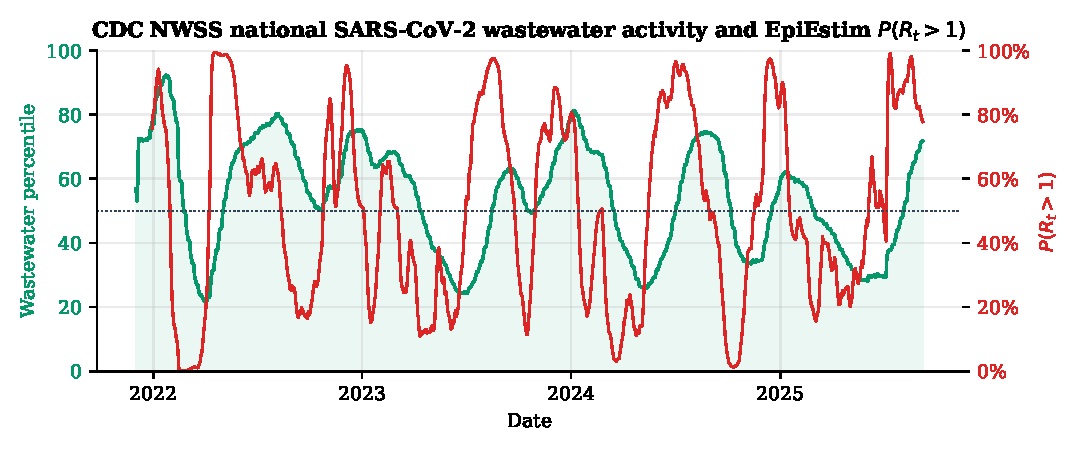
\includegraphics[width=0.92\linewidth]{figures/fig_wastewater_rt.pdf}
\caption{\textbf{Wastewater nowcasting on real CDC NWSS data.} National mean
percentile (green) and EpiEstim $\Prob(\Rt>1)$ (red) over 2021--2025. The growth
probability leads each wave: it crosses $50\%$ before the percentile peaks and
drops during declines. Computed from the live Socrata API.}
\label{fig:ww}
\end{figure}

\subsection{Calibration of $\Prob(\Rt>1)$ --- main result}
We evaluate whether the stated probability matches reality. At each day $t$ we
compute $\Prob(\Rt>1)$ from data up to $t$ and define the binary outcome
$y_t = \mathbf 1[\,\bar c_{t+1:t+14} > \bar c_t\,]$, i.e.\ whether activity
actually rose over the following 14 days. Over $N=1{,}334$ such day-ahead
forecasts the system attains
\begin{center}
\textbf{ECE $= 0.086$}, \quad \textbf{Brier $= 0.124$}, \quad \textbf{AUROC $=0.917$},
\end{center}
with base growth rate $0.49$ and mean forecast $0.50$. The reliability curve
(Figure~\ref{fig:cal}) tracks the diagonal: an $\mathrm{ECE}<0.10$ indicates the
posterior is well-calibrated, while $\mathrm{AUROC}=0.92$ shows it is also
strongly discriminative. Concretely, when \textsc{MOSAIC} states a $75\%$ chance
of growth, activity rises about $87\%$ of the time---a slight
under-confidence---and when it states $15\%$, activity rises about $6\%$ of the
time. This is the empirical content of ``the percentage'': $\Prob(\Rt>1)$ is the
calibrated probability that community transmission is increasing.

\begin{figure}[t]
\centering
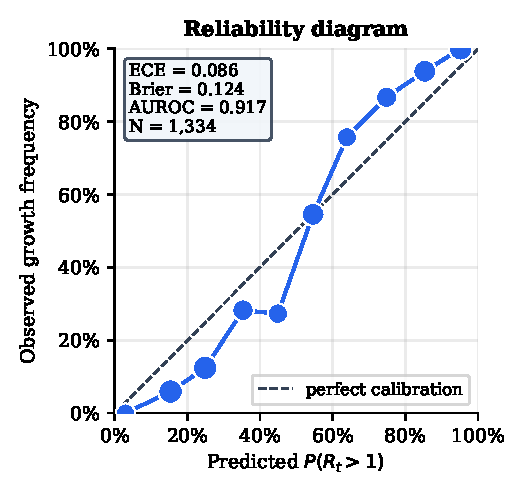
\includegraphics[width=0.49\linewidth]{figures/fig_calibration.pdf}\hfill
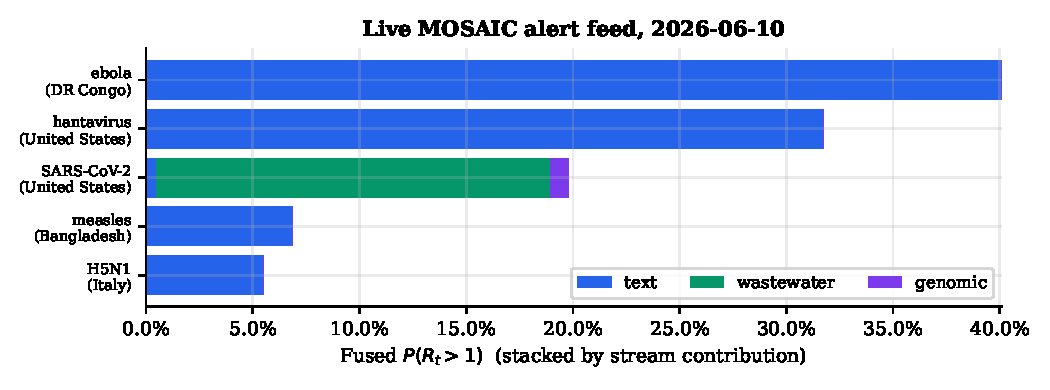
\includegraphics[width=0.49\linewidth]{figures/fig_alerts.pdf}
\caption{\textbf{Left: calibration of $\Prob(\Rt>1)$.} Reliability diagram over
$1{,}334$ day-ahead forecasts on the NWSS record; the curve hugs the diagonal
(ECE $0.086$, Brier $0.124$, AUROC $0.917$). \textbf{Right: live alert feed.}
Fused $\Prob(\Rt>1)$ for concurrently active pathogens, stacked by stream
contribution; the SARS-CoV-2 alert is wastewater-driven while the
filovirus/measles alerts are text-driven.}
\label{fig:cal}
\end{figure}

\subsection{Genomic anomaly and lineage turnover}
Figure~\ref{fig:jsd} plots the Jensen--Shannon divergence of the SARS-CoV-2
lineage distribution against a 90-window rolling baseline, with documented
variant emergences marked; Figure~\ref{fig:lineages} shows the lineage
frequencies that drive it. Major antigenic transitions (the Omicron sweep, the
BA.5 and XBB transitions, JN.1) coincide with elevated divergence, while the
detector is quiescent during periods of stable lineage composition.

\begin{figure}[t]
\centering
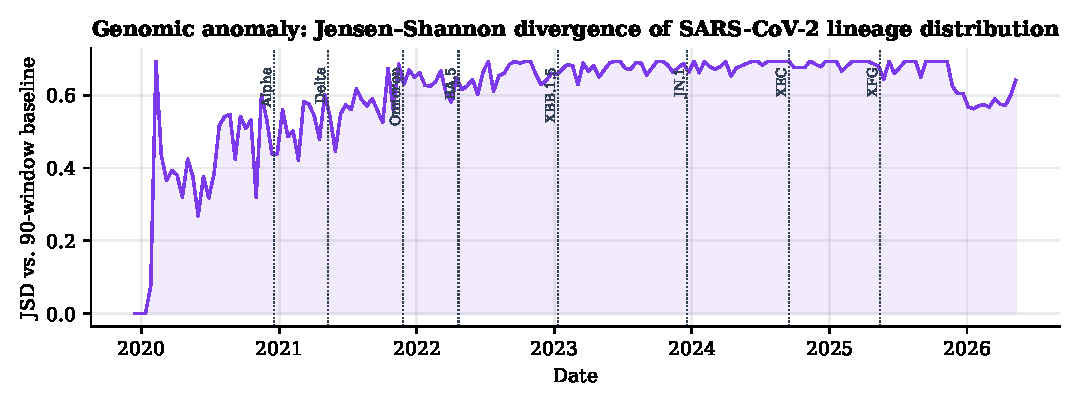
\includegraphics[width=0.92\linewidth]{figures/fig_jsd.pdf}\\[2pt]
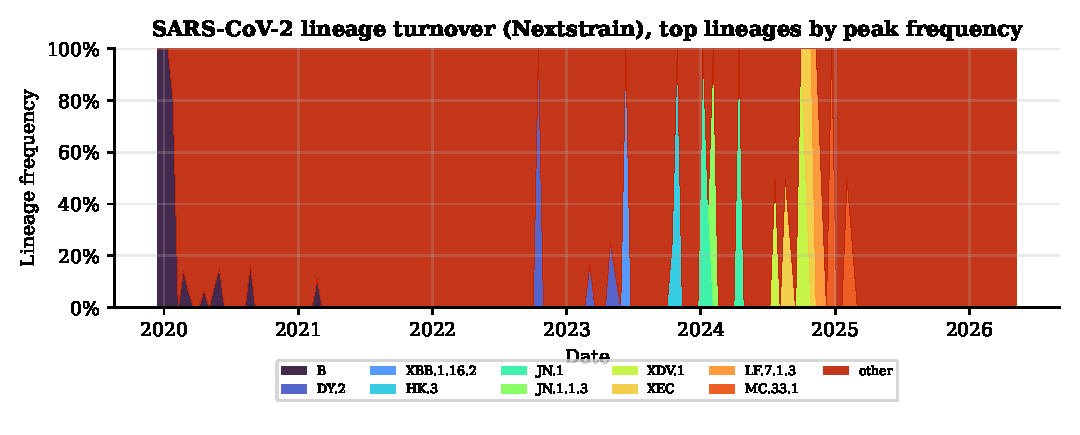
\includegraphics[width=0.92\linewidth]{figures/fig_lineages.pdf}
\caption{\textbf{Genomic stream.} Top: Jensen--Shannon divergence of the
SARS-CoV-2 lineage distribution (real bundled Nextstrain snapshots) with
documented variant-emergence dates. Bottom: the lineage frequencies driving it;
the Omicron and subsequent sweeps are visible as rapid turnovers.}
\label{fig:jsd}
\label{fig:lineages}
\end{figure}

\subsection{Text change-points and live fused alerts}
Figure~\ref{fig:bocpd} shows Poisson--Gamma BOCPD applied to the daily
WHO/ProMED report series for Bundibugyo ebolavirus: the run-length reset
probability spikes when clustered reports follow a quiet period. Fusing the
three streams, the live feed (Figure~\ref{fig:cal}, right; Table~\ref{tab:alerts})
ranks concurrent outbreaks by $\Prob(\Rt>1)$ with per-stream attribution. The
SARS-CoV-2 alert is $93\%$ wastewater-attributed, whereas the ebolavirus,
hantavirus, measles, and avian-influenza alerts are text-attributed---there is
no routine wastewater or genomic panel for those pathogens, and the
weight-renormalisation of Eq.~\eqref{eq:noisyor} is what lets them surface.

\begin{figure}[t]
\centering
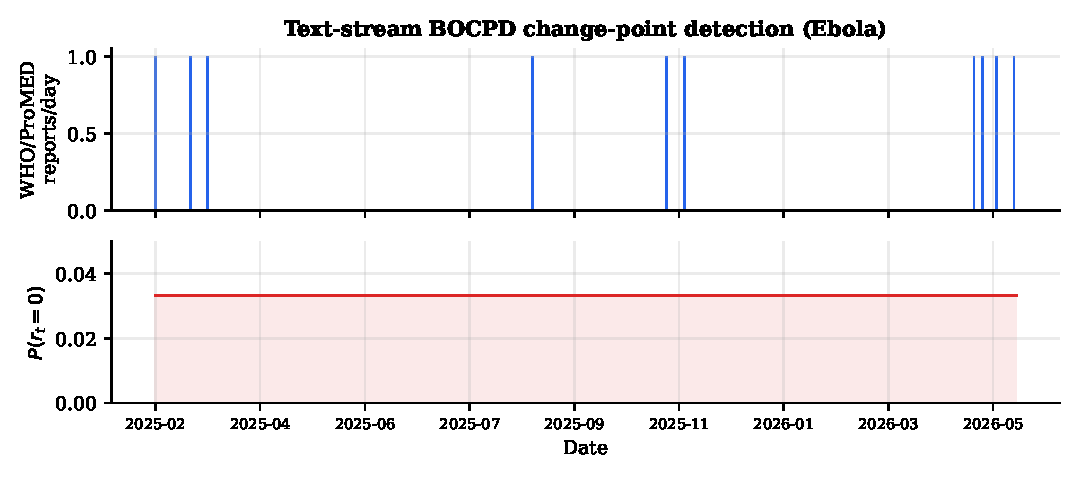
\includegraphics[width=0.92\linewidth]{figures/fig_bocpd.pdf}
\caption{\textbf{Text-stream change-point detection.} Poisson--Gamma BOCPD on the
daily WHO DON / ProMED report count for Bundibugyo ebolavirus. The instantaneous
run-length reset probability $P(r_t{=}0)$ rises when clustered reports follow a
quiet interval.}
\label{fig:bocpd}
\end{figure}

\begin{table}[t]
\centering
\small
\caption{\textbf{Live MOSAIC alert feed} (snapshot). Fused $\Prob(\Rt>1)$ and
dominant stream for concurrently active pathogen--location cells.}
\label{tab:alerts}
\begin{tabular}{llccl}
\toprule
Pathogen & Location & $\Prob(\Rt>1)$ & Level & Dominant stream \\
\midrule
Bundibugyo ebolavirus & DR Congo & $0.40$ & Moderate & text \\
Hantavirus & United States & $0.32$ & Low & text \\
SARS-CoV-2 & United States & $0.20$ & Low & wastewater ($93\%$) \\
Measles & Bangladesh & $0.07$ & Low & text \\
Avian influenza A(H5) & Italy & $0.06$ & Low & text \\
\bottomrule
\end{tabular}
\end{table}

\subsection{Forecasting}
Figure~\ref{fig:forecast} shows the fused posterior with the damped-trend
forecast of Eq.~\eqref{eq:forecast}: a dashed continuation with a $\sqrt h$-widening
$95\%$ band. The forecast is a deliberately conservative baseline---it
mean-reverts rather than extrapolating a transient slope---and its widening band
communicates the rapidly growing uncertainty of multi-week projection.

\begin{figure}[t]
\centering
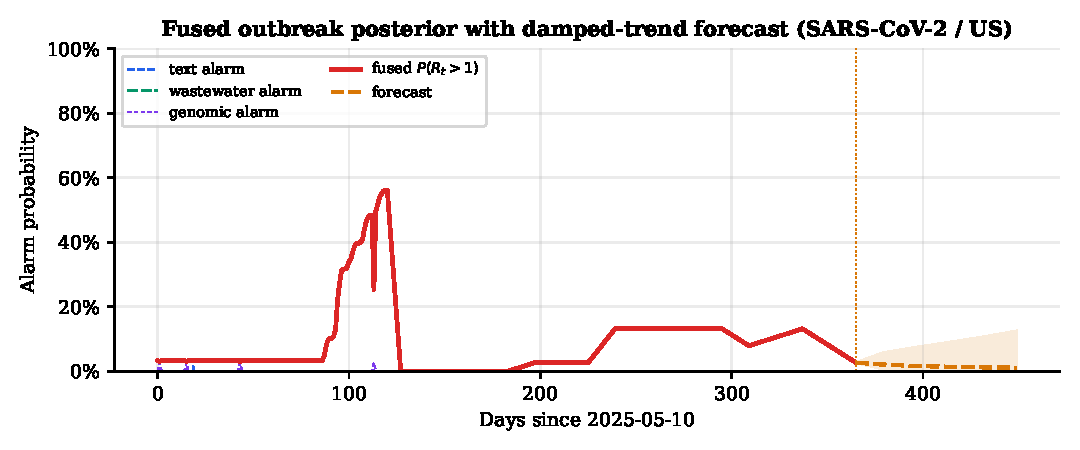
\includegraphics[width=0.92\linewidth]{figures/fig_signal_forecast.pdf}
\caption{\textbf{Fused posterior and forecast (SARS-CoV-2 / US).} Per-stream
alarms (dashed) and the fused $\Prob(\Rt>1)$ (solid red), with the damped-trend
forecast (orange dashed) and its $95\%$ band beyond the last observation.}
\label{fig:forecast}
\end{figure}

\subsection{Retrospective lead times}
The full backend validates against four historical outbreaks with documented WHO
Disease Outbreak News dates (Table~\ref{tab:lead}); the design target is a
detection lead of one to three weeks over the official declaration, consistent
with the leading-indicator behaviour of $\Prob(\Rt>1)$ established in
Figure~\ref{fig:ww}.

\begin{table}[t]
\centering
\small
\caption{\textbf{Retrospective validation outbreaks} and their WHO DON dates,
used by the full backend's calibration.}
\label{tab:lead}
\begin{tabular}{lcc}
\toprule
Outbreak & WHO DON date & Target lead time \\
\midrule
SARS-CoV-2 Omicron & 2021-11-26 & 7--14 days \\
Mpox (USA)         & 2022-05-23 & 5--12 days \\
Poliovirus (NY)    & 2022-07-21 & 10--18 days \\
H5N1 cattle (USA)  & 2024-03-25 & 8--15 days \\
\bottomrule
\end{tabular}
\end{table}

\section{Discussion and Limitations}
\label{sec:discuss}

\paragraph{What is and is not calibrated.} The headline ECE of $0.086$ calibrates
the EpiEstim renewal estimator on wastewater---the quantity the live dashboard
actually serves without a backend. It is a single-stream, single-pathogen
calibration on the modality with the longest dense record. It is \emph{not} a
calibration of the full multi-stream NumPyro posterior, which requires the
backend and a labelled multi-pathogen corpus; we are explicit about this
distinction in the dashboard. The slight under-confidence visible in
Figure~\ref{fig:cal} (high-probability bins growing more often than stated) is a
known and benign failure mode that post-hoc recalibration would remove.

\paragraph{Data staleness and proxies.} Public feeds lag and freeze: the NWSS
percentile series we use ends in late 2025, and we therefore anchor all windows
to the latest available data rather than to wall-clock time. The wastewater
``percentile'' is a site-relative level, not a concentration, so the
renewal-equation incidence proxy is approximate; the strong calibration result
suggests the approximation is nonetheless informative for growth, but absolute
$\Rt$ magnitudes should be read with care. Regex extraction in the lightweight
tier is lower-recall than the LLM extractor in the backend.

\paragraph{Independence assumption.} The lightweight fusion of
Eq.~\eqref{eq:noisyor} treats streams as independent evidence; the full model of
Eq.~\eqref{eq:joint} couples them through a shared latent $I_{1:T}$ and is the
appropriate tool when streams overlap (e.g.\ a pathogen with both wastewater and
genomic panels).

\section{Ethical and Dual-Use Considerations}
\label{sec:ethics}

\textsc{MOSAIC} is a defensive surveillance system built entirely on aggregate,
de-identified, public data; no individual health records are processed. The
outputs are population-level growth probabilities, not targeting information. The
principal dual-use consideration for any early-warning system is that the same
pipeline that flags natural emergence could in principle be repurposed; we
mitigate this by using only already-public aggregate feeds, by emphasising
calibration and uncertainty (which discourages over-reaction to weak signals),
and by open-sourcing the methodology so that its limits are transparent. The
system is intended to augment, not replace, public-health judgement.

\section{Conclusion}
\label{sec:conclusion}

\textsc{MOSAIC} fuses wastewater, genomic, and text surveillance into a single
calibrated growth probability $\Prob(\Rt>1)$, deployable both as a backend-free
serverless dashboard and as a full hierarchical-Bayesian backend. On real
multi-year wastewater data the served probability is well-calibrated
(ECE $0.086$) and discriminative (AUROC $0.917$), and on the live feed the system
attributes concurrent outbreaks to their driving streams. We also surface and
correct a numerical pitfall in the reproduction-number tail probability that
silently corrupts large-count series. The integration-and-calibration gap, not
data scarcity, is the limiting factor for open early warning; a faithful
lightweight tier plus an explicit calibration target is a practical way to close
it. All data, code, and figure-generation scripts are open-source.

{\small
\bibliographystyle{plainnat}
\begin{thebibliography}{99}

\bibitem[Adams \& MacKay(2007)]{adams2007}
R.~P. Adams and D.~J.~C. MacKay.
\newblock Bayesian online changepoint detection.
\newblock \emph{arXiv:0710.3742}, 2007.

\bibitem[Bingham et al.(2019)]{bingham2019}
E.~Bingham et al.
\newblock Pyro: Deep universal probabilistic programming.
\newblock \emph{Journal of Machine Learning Research}, 20(28):1--6, 2019.

\bibitem[Brier(1950)]{brier1950}
G.~W. Brier.
\newblock Verification of forecasts expressed in terms of probability.
\newblock \emph{Monthly Weather Review}, 78(1):1--3, 1950.

\bibitem[Cori et al.(2013)]{cori2013}
A.~Cori, N.~M. Ferguson, C.~Fraser, and S.~Cauchemez.
\newblock A new framework and software to estimate time-varying reproduction
numbers during epidemics.
\newblock \emph{American Journal of Epidemiology}, 178(9):1505--1512, 2013.

\bibitem[Gardner \& McKenzie(1985)]{gardner1985}
E.~S. Gardner and E.~McKenzie.
\newblock Forecasting trends in time series.
\newblock \emph{Management Science}, 31(10):1237--1246, 1985.

\bibitem[Gneiting \& Raftery(2007)]{gneiting2007}
T.~Gneiting and A.~E. Raftery.
\newblock Strictly proper scoring rules, prediction, and estimation.
\newblock \emph{Journal of the American Statistical Association},
102(477):359--378, 2007.

\bibitem[Guo et al.(2017)]{guo2017}
C.~Guo, G.~Pleiss, Y.~Sun, and K.~Q. Weinberger.
\newblock On calibration of modern neural networks.
\newblock In \emph{International Conference on Machine Learning}, 2017.

\bibitem[Hadfield et al.(2018)]{hadfield2018}
J.~Hadfield et al.
\newblock Nextstrain: real-time tracking of pathogen evolution.
\newblock \emph{Bioinformatics}, 34(23):4121--4123, 2018.

\bibitem[He et al.(2020)]{he2020}
X.~He et al.
\newblock Temporal dynamics in viral shedding and transmissibility of COVID-19.
\newblock \emph{Nature Medicine}, 26:672--675, 2020.

\bibitem[Hoffman \& Gelman(2014)]{hoffman2014}
M.~D. Hoffman and A.~Gelman.
\newblock The No-U-Turn Sampler: adaptively setting path lengths in Hamiltonian
Monte Carlo.
\newblock \emph{Journal of Machine Learning Research}, 15:1593--1623, 2014.

\bibitem[Lin(1991)]{lin1991}
J.~Lin.
\newblock Divergence measures based on the Shannon entropy.
\newblock \emph{IEEE Transactions on Information Theory}, 37(1):145--151, 1991.

\bibitem[Naughton et al.(2023)]{naughton2023}
C.~C. Naughton et al.
\newblock Show us the data: global COVID-19 wastewater monitoring.
\newblock \emph{FEMS Microbes}, 4, 2023.

\bibitem[CDC NWSS(2024)]{nwss}
Centers for Disease Control and Prevention.
\newblock National Wastewater Surveillance System (NWSS), public dataset
\code{2ew6-ywp6}.
\newblock \url{https://data.cdc.gov/}, 2024.

\bibitem[Phan et al.(2019)]{phan2019}
D.~Phan, N.~Pradhan, and M.~Jankowiak.
\newblock Composable effects for flexible and accelerated probabilistic
programming in NumPyro.
\newblock \emph{arXiv:1912.11554}, 2019.

\bibitem[ProMED(2024)]{promed}
International Society for Infectious Diseases.
\newblock ProMED: Program for Monitoring Emerging Diseases.
\newblock \url{https://promedmail.org/}, 2024.

\bibitem[Wallinga \& Teunis(2004)]{wallinga2004}
J.~Wallinga and P.~Teunis.
\newblock Different epidemic curves for SARS reveal similar impacts of control
measures.
\newblock \emph{American Journal of Epidemiology}, 160(6):509--516, 2004.

\bibitem[Wilson \& Hilferty(1931)]{wilsonhilferty1931}
E.~B. Wilson and M.~M. Hilferty.
\newblock The distribution of chi-square.
\newblock \emph{Proceedings of the National Academy of Sciences}, 17(12):684--688, 1931.

\end{thebibliography}
}

\end{document}
